\section{Quest - Selection}
%TODO Referenz Quest System

Sobald ein Package ausgewählt wurde, kann man darin die Quest wählen. Wie beim Questpackage wird rechts die Beschreibung der ausgewählten Quest angezeigt. Der \textbf{"`Type"'} kann in der \textbf{quest.xml} definiert werden. Somit kann man zum Beispiel für verschiedene Aufgabenbereiche verschiedene Attribute verwenden. Links wird der Status der jeweiligen Quest in Symbolen dargestellt.

\begin{figure}[h] 
  \centering
     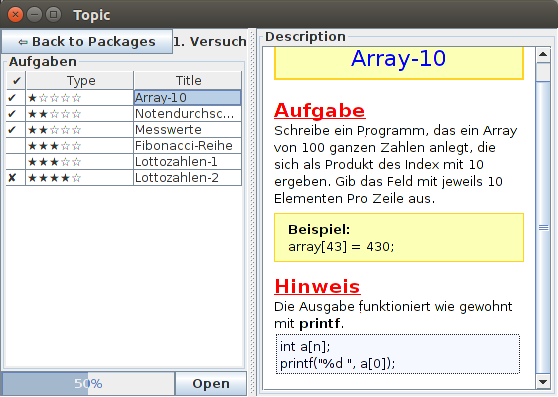
\includegraphics[width=0.9\textwidth]{./media/images/gui/launcher/package_view.png}
  \caption{Quest Selection}
  \label{fig:Bild1}
\end{figure}

\begin{itemize}
\item Mit einem leeren Feld wird eine nicht gestartete Quest symbolisiert.
\item Eine Uhr bedeutet, dass die Quest bereits gestartet, jedoch noch nicht abgeschlossen wurde.
\item Ein Häkchen symbolisiert eine fertiggestellte Quest.
\item Ein Kreuz bedeutet eine gesperrte Quest. 
\end{itemize}

Die Questzustände werden im Kapitel \ref{sec:Queststate} genauer erklärt.

Sobald eine Quest selektiert wurde, wird der grau hinterlegte \textbf{"`Open"'} Button aktiv und kann nun geklickt werden. Sobald dies geschehen ist, wird die gewählte Quest als aktuelle Quest ins Profil übernommen und C Compact dementsprechend angepasst. Die Quest wird somit gestartet.

Zur Realisierung wurde eine JTable verwendet. Diese befindet sich wiederum in einer JScrollpane. Das Questpackage und die Questselection verwenden grundsätzlich dasselbe JFrame. Beim Wechseln auf die JTable, muss die JTreeTable entfernt werden. Danach kann der neue JTable hinzugefügt werden.
\begin{lstlisting}[language=JAVA]
	public void changetoQuestTable(){
		splitpane.remove(jTablePanel);
		splitpane.setLeftComponent(inittable());

		frame.validate();
		frame.repaint();
	}
\end{lstlisting}

%Mithilfe der \textit{frame.validate()} Methode wird noch einmal überprüft, ob alle Komponenten ordnungsgemäß zugewiesen werden. Danach muss das gesamte JFrame neu gezeichnet werden, was in diesem Fall von der \textit{frame.repaint()}-Methode durchgeführt wird.